\section{Planificacion}
\label{Planificacion}

    El proyecto abarca una carga docente estipulada de 12 ECTS, equivalente a 300 horas de dedicación en el plan de estudios del Grado en Informática. El cronograma cubre la toma inicial de requisitos, el modelado del dominio, la codificación del sistema distribuido, la integración de modelos de lenguaje y la redacción de la memoria. La figura~\ref{fig:planificacion_temporal_general} recoge la descomposición temporal de este trabajo.

    El trabajo preliminar absorbió 100 horas repartidas durante el primer mes: evaluación tecnológica (30 horas), especificación de requisitos del sistema (30 horas) y diseño de maquetas de interfaz (40 horas). Esta fase sirvió para contrastar la viabilidad del protocolo MCP con Spring AI, verificar la velocidad de inferencia del proveedor Groq, normalizar las tablas en PostgreSQL y cerrar los flujos de navegación antes de codificar la solución.

    El núcleo de programación concentró 170 horas de esfuerzo. La construcción de la aplicación web y los microservicios acaparó 110 horas, programando la lógica de negocio en Spring Boot 3, el cliente web en React con TanStack Query y el servidor MCP en Node.js. Sobre esta base funcional se desarrollaron tres hitos derivados: el empaquetado móvil sobre Android con Capacitor (25 horas), la definición de contenedores Docker y el despliegue en la nube de Microsoft Azure (20 horas), y una batería final de pruebas de integración con JUnit y Mockito (15 horas) para verificar la consistencia transaccional y la autenticación sin estado.

    Las 30 horas finales se asignaron a redactar la memoria en LaTeX conforme a las pautas tipográficas de la Escuela Superior de Ingeniería, generar los diagramas formales en PlantUML y preparar la defensa ante el tribunal. La redacción se abordó con el software ya estabilizado, garantizando que el texto reflejara el comportamiento exacto de las rutas, entidades y eventos implementados.

\begin{figure}[htbp]
    \centering
    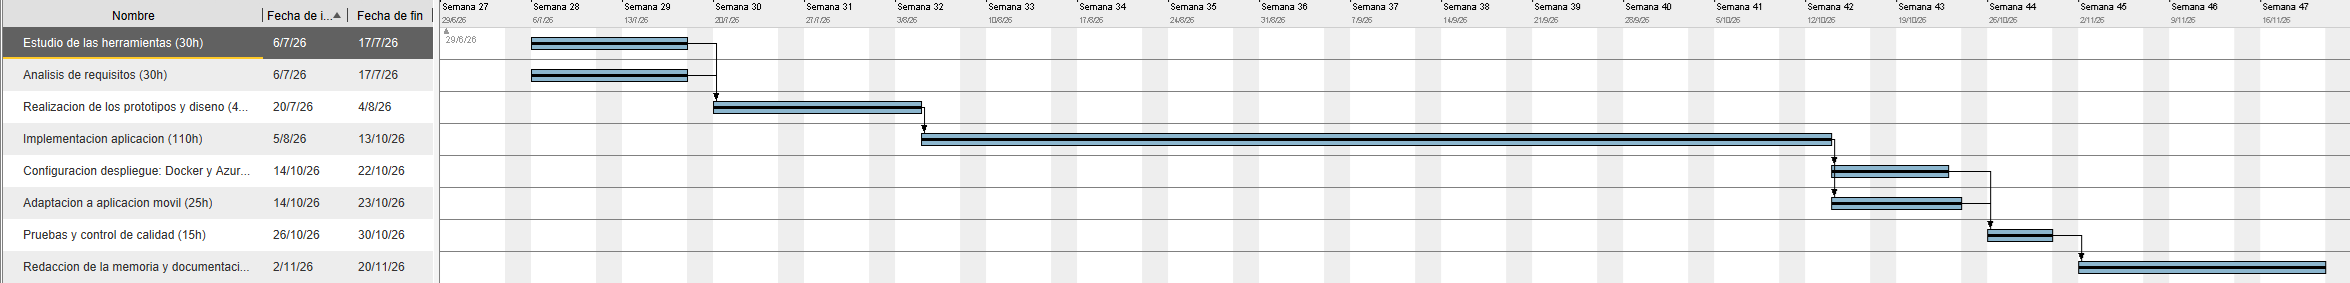
\includegraphics[width=0.85\textwidth]{Introduccion/img/Planificacion.png}
    \caption{Planificación Temporal General}
    \label{fig:planificacion_temporal_general}
\end{figure}

    Las 110 horas dedicadas al desarrollo exigieron planificar qué módulos podían ejecutarse en paralelo y cuáles imponían una secuencia obligatoria por dependencias de datos.

    El trabajo simultáneo aceleró las capas base: mientras se levantaban las entidades JPA y las migraciones en PostgreSQL, se maquetaba el armazón de rutas y componentes en React con Tailwind CSS. La autenticación local mediante tókenes JWT y el inicio de sesión federado con Google OAuth se construyeron en paralelo a sus formularios web en el cliente. De igual manera, el buscador de alojamientos avanzó al mismo tiempo que el mapa interactivo de Leaflet, pues ambas vistas consumían los mismos endpoints REST del backend.

    Las reglas de negocio troncales requirieron un avance estrictamente secuencial debido a restricciones del modelo relacional:

\begin{enumerate}
    \item \textbf{Gestión de alojamientos y catálogo}: habilitó la persistencia de propiedades, la subida de fotografías a Cloudinary y la definición de comodidades antes de admitir cualquier interacción.
    \item \textbf{Solicitudes de reserva y cobro de fianza}: se apoyó en el catálogo activo para gestionar rangos de fechas sin colisiones temporales y conciliar el abono de la fianza.
    \item \textbf{Espacio del hogar}: se instanció como contenedor lógico derivado de una reserva confirmada y abonada, agrupando a los inquilinos aceptados.
    \item \textbf{Gastos compartidos y tareas domésticas}: dependían de la existencia previa del hogar. Se implementó el motor de saldos contables con simplificación de deudas y, tras verificarlo, se programó el reparto rotativo de limpieza con asignaciones periódicas y recompensas.
    \item \textbf{Mensajería contextual}: se construyó sobre la convivencia constituida, permitiendo conversaciones entre compañeros de piso o entre inquilinos y propietarios.
    \item \textbf{Asistente virtual (Spring AI y MCP)}: se integró tras estabilizar los endpoints de catálogo y tareas, permitiendo que el servidor MCP consumiera datos consolidados sin lidiar con contratos cambiantes en la API interna.
    \item \textbf{Moderación, valoraciones y RGPD}: cerró el sistema antes de la fase de despliegue, añadiendo denuncias disciplinarias, reseñas mutuas y políticas de supresión de datos personales.
\end{enumerate}

\begin{figure}[htbp]
    \centering
    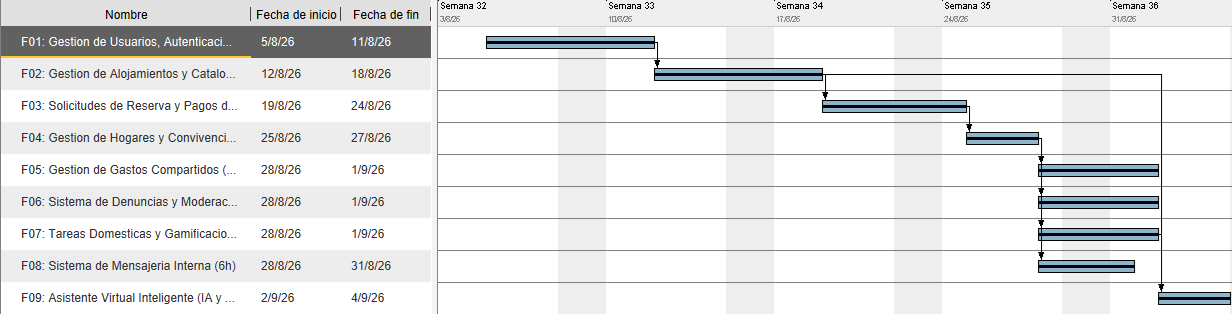
\includegraphics[width=0.85\textwidth]{Introduccion/img/planificacionImplementacion.png}
    \caption{Planificación Temporal de la implementación}
    \label{fig:planificacion_temporal_implementacion}
\end{figure}